%Review of timbral control research.
%	Timbre Definition
%	Timbre Spaces (MDS and shit)
%	Audio Features
%	Perceptual Control of Synthesis

\chapter{Timbre}
\label{chap:Timbre}
\note
{
	CataRT system developed by \citet{schwarz2007corpus}.

	Temporal features, hidden markov models to look at feature change over time. 

	All that stuff about only distorting the only the sustain.

	Timbral effects of amplitude envelope being reversed \citep{patterson1994the}.

}

\section{Introduction}
\label{sec:Timbre-Introduction}
	There are three properties which describe how a sound is perceived, these being loudness, pitch and timbre.
	Loudness describes the perceived intensity of a sound and pitch its perceived frequency. Timbre then describes any
	other properties of a sound, besides loudness and pitch, which allow it to be distinguished from other sounds
	\citep{mathews1999introduction}. Loudness and pitch are both one dimensional properties allowing sounds to be
	ordered from quiet to loud or low to high pitch. Timbre is a more complex property consisting of multiple
	dimensions \citep{rossing2002the}. There is a large body of research concerning the analysis of timbre, identifying
	these dimensions and their relationships with the acoustic features of a sound.

	\note
	{
		better introduce this paragraph (layman's description)
	}

	Simple descriptions of a sounds timbre involve instrument identification. A sound could be described as
	`cello-like' or `flute-like'. More broadly the class of instrument, string or woodwind, could be used to describe
	the timbre of a sound. While these terms are useful for discussing the instrumentation of pieces they can not be
	applied generally to a wide range of timbres. It is not very useful to describe the timbre of a xylophone as being
	`not flute-like'.

	More general timbral descriptors directly describe the sound itself rather than the source which produced it. These
	include terms such as bright, rough and sharp. This allows the timbre of different sounds to be compared according
	to these terms \citep{howard2009acoustics}. Sounds can also be ordered in respect to these criteria much like with
	loudness and pitch. For example one could order a set of sounds by how bright they sound.

	Early research into timbre was performed by \citet{helmholtz1875on}. More recent work involves research from
	various fields. Low level features of audio segments can be found using signal analysis techniques. More
	complicated information about the perception of a signal can be discovered through modelling the behaviour of the
	human hearing system. Lastly experiments can be undertaken in which participants listen to audio stimuli and
	provide responses regarding the their timbre. These responses are then analysed to uncover any correlations between
	the participants responses and lower level features of the stimuli.

	This chapter will review the existing body of timbral research. Section \ref{sec:Timbre-LowLevelFeatures} discusses
	metric which are used to describe the low level features of audio signals. Section
	\ref{sec:Timbre-PsychoacousticPrinciples} covers various models which describe the perception of various auditory
	phenomena. \note{Put in what the rest of the sections are about}.

	\note
	{
		discuss where the current vocabulary comes from and the general world of timbre description

		discuss state of the art and where this thesis takes on from that
	}

\section{Low Level Audio Features}
\label{sec:Timbre-LowLevelFeatures}
	A widely cited definition of timbre \citep{ASA1960american} suggests that timbre in influenced by various low level
	features of an audio signal. The spectral content, waveform and temporal characteristics all effect the perceived
	timbre of a sound. Signal analysis techniques can be used to extract information about these elements of a signal.
	A large list of such feature extraction techniques is given by \citet{peeters2004a} and
	\citet{bullock2008implementing}. These features can be separated into three categories. Features which describe the
	properties of a signal's waveform and how it evolves with time (temporal features), features which describe the
	frequency content of a signal (spectral features) and features which describe how the frequency content of a signal
	evolves with time (spectro-temporal features). In the later part of this work (Chapters \ref{chap:TimbreEvaluation}
	and \ref{chap:FeatureControl}) several of these features are discussed in the analysis of timbre and operation of
	audio effects. Definitions for the features discussed in those chapters are given in this section, for definitions
	of other audio features refer to the previously published literature \citep{peeters2004a, bullock2008implementing}.

	\subsection{Temporal Features}
	\label{sec:Timbre-LowLevelFeatures-Temporal}
		Simple temporal features involve taking statistical measurements, such as mean and variance, of the audio
		samples in a signal. These measures give basic information about the amplitude of samples in a signal vary,
		but in many cases they do not represent a signals properties very well. For example, the mean value of a
		sinusoidal signal over a whole number of cycles is zero. A common technique to extract more meaningful
		information about a signals level is to use an envelope detector. An envelope detector produces an envelope
		for a signal: a smooth line which describes the peaks or troughs in a signal, ignoring the oscillatory
		changes in amplitude due to its frequency. Applying an envelope detector to the temporal representation of
		a signal produces an amplitude envelope describing the level of the signal over time. Figure
		\ref{fig:AmplitudeEnvelope} illustrates the amplitude envelope of a simple signal.

		\begin{figure}[h!]
			\centering
			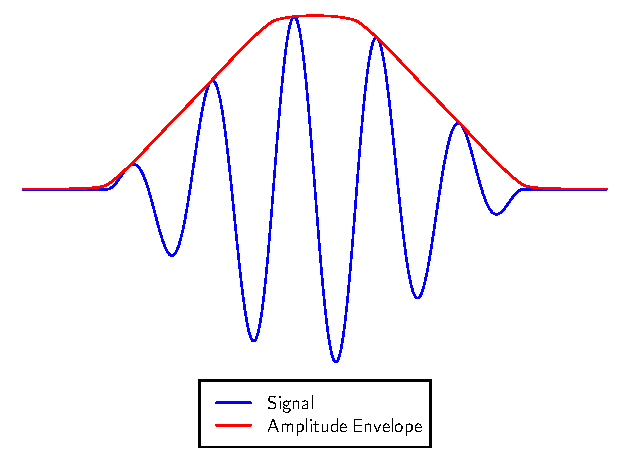
\includegraphics{chapter2/Images/AmplitudeEnvelope.pdf}
			\caption{The amplitude envelope of a signal.}
			\label{fig:AmplitudeEnvelope}
		\end{figure}

		\subsubsection*{Envelope Detection}
			Simple envelope detectors can be implemented based on those used in electronic circuits. First
			rectification is applied to produce a unipolar signal and then a low pass filter is applied to
			smooth the result \citep{dutilleux2011modulators}. In the digital domain more complex envelope
			detectors are possible such as the instantaneous amplitude detector. Instantaneous amplitude is
			calculated as the absolute value of an analytic representation of the input signal. An analytic
			signal is a complex valued signal, the real part of which is the original signal and the imaginary
			part its Hilbert transform. The analytic signal is often denoted with a subscript letter $a$, such
			that the analytic representation of the signal $x[n]$ would be denoted $x_{a}[n]$. This method and
			more complex digital envelope detectors are reviewed by \citet{chang2007a}. 

			Implementing an instantaneous amplitude detector involves making performance compromises. An ideal
			Hilbert transform alters the phase information of a signal while leaving the magnitude information
			unchanged. Any negative frequencies in the signal have their phase shifted by $\frac{\pi}{2}$
			radians while the phase of positive frequencies is shifted by $-\frac{\pi}{2}$ radians. The
			transfer function for an FIR implementation of a Hilbert transform is shown in Equation
			\ref{eq:FirHilbertTransform}.

			\begin{equation}
				H(z) = \sum_{m = -M}^{M} \frac{2}{m\pi} sin^{2} \left( \frac{m\pi}{2} \right) z^{-m}
				\label{eq:FirHilbertTransform}
			\end{equation}

			For an ideal Hilbert transform the impulse response should be infinitely long ($M = \infty$).
			Practicable approximations of an ideal Hilbert transform can be created by using a finite value for
			$M$. A delay of $M$ samples must also be introduced in order to give a causal filter. As the value
			of $M$ is decreased this delay is reduced while the magnitude response of the filter deviates
			further from the ideal. Figure \ref{fig:HilbertMagnitude} shows the magnitude responses for FIR
			Hilbert transform filters with $M = 11$ and $M = 101$. The filters have a bandpass response with
			some ripple in the pass band. As $M$ is increased the bandwidth of the passband is increased and
			the ripple reduced. The phase response of these filters remains ideal no matter the value of $M$,
			as evidenced by Figure \ref{fig:HilbertPhase}.

			\begin{figure}[h!]
				\centering
				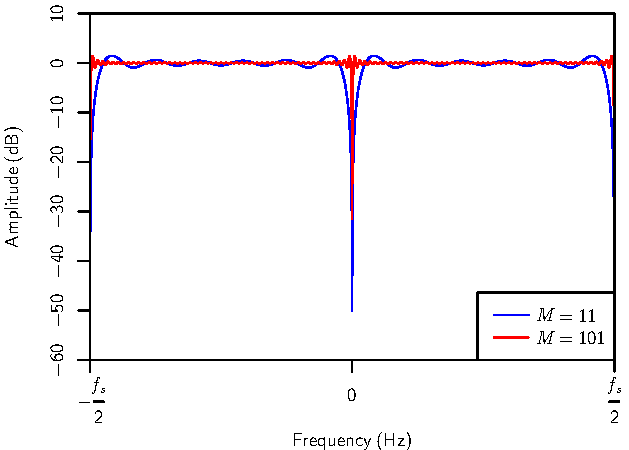
\includegraphics{chapter2/Images/HilbertMagnitudeResponses.pdf}
				\caption{Magnitude responses of FIR Hilbert transform filter with different orders.}
				\label{fig:HilbertMagnitude}
			\end{figure}

			\begin{figure}[h!]
				\centering
				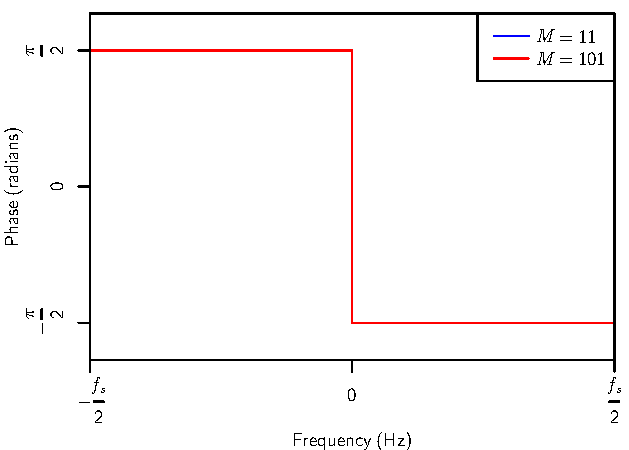
\includegraphics{chapter2/Images/HilbertPhaseResponses.pdf}
				\caption{Phase responses of FIR Hilbert transform filters with different orders.}
				\label{fig:HilbertPhase}
			\end{figure}

			When using Equation \ref{eq:FirHilbertTransform} a compromise needs to be made between the
			tolerable amount of delay and the accuracy of the filter's magnitude response. Increasing $M$ will
			give a more accurate filter but introduce more delay and increase the complexity of the filter.
			More efficient implementations can be built using IIR filters if some of the properties of an ideal
			Hilbert transform are disregarded.  \citet{oppenheim2014discrete} suggest constructing a phase
			splitter: processing audio with two parallel allpass IIR filters the phase responses of which
			differ from each other by $\frac{\pi}{2}$ radians for a large proportion of the spectrum. While
			this is not strictly a Hilbert transform it creates two signals which can be used as the real and
			imaginary part of an analytic signal. \citet{niemitalo2003hilbert} provides an implementation of
			such a pair of filters. The phase difference between these two filters is seen in Figure
			\ref{fig:IIRHilbertPhase}.

			\begin{figure}[h!]
				\centering
				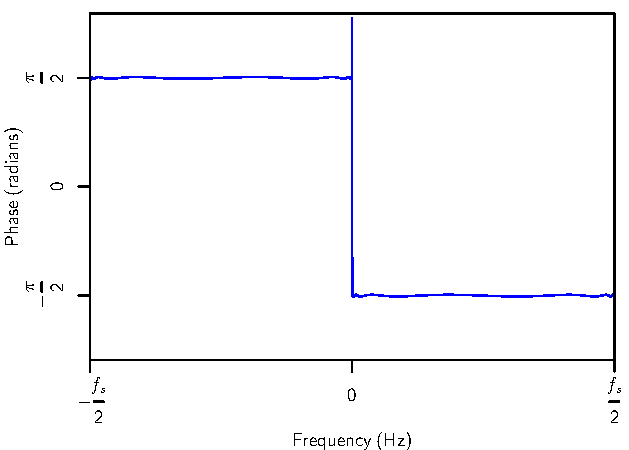
\includegraphics{chapter2/Images/IIRHilbertPhaseResponses.pdf}
				\caption{The phase difference between the two allpass filters proposed by
					 \citet{niemitalo2003hilbert}.}
				\label{fig:IIRHilbertPhase}
			\end{figure}

		\subsubsection*{Amplitude Envelope Analysis}
			The amplitude envelope of a signal can be used to extract more meaningful information about it's
			temporal evolution. This is often done by splitting the sound into different sections according to
			the properties of its amplitude envelope. \citet{howard2009acoustics} separates the amplitude
			envelope of a sound into three sections: the steady state section being the middle portion in which
			the timbre of the sound only varies slightly and the onset and offset sections which describe the
			way the sound rises from silence to the steady state and returns to silence afterwards. Further
			refinement of the description of amplitude envelopes leads to the ADSR (Attack, Decay, Sustain,
			Release) model \citep{descrivan2012music}. The attack and decay portions constitute the onset of
			the signal, the attack describing the time it takes for the amplitude to rise from silence to a
			maximum and the decay describing the time it takes for the amplitude to decrease back to a steady
			level. The sustain describes the level at which the amplitude remains during the steady state
			portion of the signal and the release the time taken for the amplitude to fall from this level to
			silence. An example ADSR envelope is shown in Figure \ref{fig:ADSR}.

			\begin{figure}[h!]
				\centering
				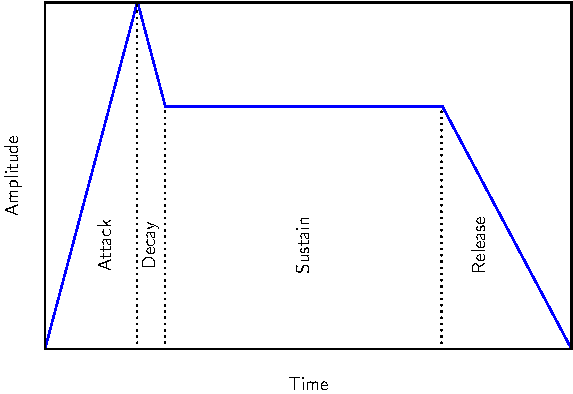
\includegraphics{chapter2/Images/ADSR.pdf}
				\caption{An ADSR envelope.}
				\label{fig:ADSR}
			\end{figure}

			Properties of the amplitude envelope can be used to describe the temporal features of a signal's
			amplitude. The attack time of sounds is important in the distinction of different timbres
			\citep{ilmoniemi2004subjective} and is often scaled logarithmically giving the log attack time.
			Other temporal features measure the amplitude envelope in its entirely, such and the temporal
			centroid which is the mean time of the signals duration weighted by the amplitude at each instant
			\citep{peeters2000instrument}.

		\subsubsection*{Other Temporal Audio Features}
			Basic frequency information can be attained trough temporal analysis by enumerating the number of
			specific events which happen in a given time period. One such event is a zero crossing (a change in
			signal polarity), the counting of which can yield an estimate of the frequency content of a signal
			(the zero crossing rate). The temporal distance between similar events in a signal can also be
			found through autocorrelation and used as an estimate of pitch / frequency \citep{mcleod2005a}.

			Larger scale temporal feature measure the properties of passages of music rather than individual
			notes, such as the measure used by \citet{wilson2014profiling} in which probability mass function
			(PMF) of sample amplitudes in a segment of audio is used as a measure of distortion present.
			Temporal features on this scale are outside of the scope of this work as they no longer relate to
			the timbre of individual sounds but rather the perceived nature of a musical piece.

	\subsection{Spectral Features}
	\label{sec:Timbre-LowLevelFeatures-Spectral}
		In existing timbral research is is widely reported that features describing a sound's spectrum produce the
		largest effects on timbre. To calculate these features the signal is first converted into a frequency
		domain representation. This is most commonly done using either the Discrete Fourier Transform (DTF) or a
		filter bank. The calculation of many spectral features is done directly from these spectral
		representations, for others peak finding is applied to the spectrum in order to determine the spectral
		partials.

		The spectral partials of a signal are its distinct frequency components. These are analogous to the
		vibrational modes of a physical body. Determining the spectral partials of a signal allows the tonal
		content of a signal to be isolated from the noise content. The noise energy in a signal describes any
		energy which is does not contribute to a spectral partial. The noisiness of a signal can be measured as the
		ratio of the noise energy to the total energy in the signal \citep{serra1998sound}.

		Further analysis can be performed by finding the harmonic partials of the signal. This requires a
		calculation of the fundamental frequency ($f_{0}$) of the signal. $f_{0}$ is a property of periodic signals
		and is equal to the inverse of the signal's period (i.e. its lowest frequency component). Harmonic partials
		of a signal are the spectral partials with frequencies which are an integer multiple of the $f_{0}$. In
		detecting the harmonic partials it is usual to allow for a slight deviation from perfect harmonic
		structure, as described by \citet{peeters2011the}.

		To aid in discussion throughout this work it is useful to define the concept of a spectral component. This
		is a general concept used to describe individual portions of a signal's spectrum. A signal is composed of
		$N$ spectral components which are each describe by an amplitude and a frequency. The amplitude and
		frequency of the $n$\super{th} spectral component are denoted $a_{n}$ and $\nu_{n}$ respectively. Spectral
		components can describe DFT bins, $a_{n}$ being the bin's magnitude and $\nu_{n}$ its frequency; filter
		bank bands, $a_{n}$ representing the total energy in the band and $\nu_{n}$ the band's center frequency; or
		spectral partials, $a_{n}$ and $\nu_{n}$ giving the amplitude and frequency of the partial. Several of the
		features discussed in this section can be calculated from any type of spectral components so this uniform
		notation proves very useful. Where the calculation of a feature requires a particular spectral
		representation this will be noted.

		Some features are calculated using the energy at harmonic frequencies within a signal. This is different to
		using the harmonic partials as the energy at harmonics which are not considered partials should still be
		included. The equations for calculating these features use a slightly different notation. Features are
		calculated from the amplitudes of the first $N$ harmonics in a signal, denoted $h_{n}$. No additional
		notation is required for the frequency of the harmonic as it is implicitly equal to $nf_{0}$Hz.

		\subsubsection*{Spectral Moments}
			The spectral moments are the statistical moments of a signals spectrum. They describe how the
			energy is distributed in a spectrum. The first four spectral moments are the centroid, spread,
			skewness and kurtosis.

			The spectral centroid of a signal, $\mu_{\textrm{s}}$, is the first raw moment (mean) of the
			spectrum. It is calculated using Equation \ref{eq:SpectralCentroid}. Spectral centroid is often
			stated as being one of the most salient audio features in timbre recognition
			\citep{freed1990auditory, lakatos2000a}. 

			\begin{equation}
				\mu_{\textrm{s}} = \frac{\sum_{n = 1}^{N} \nu_{n}a_{n}}
					   	   {\sum_{n = 1}^{N} a_{n}}
				\label{eq:SpectralCentroid}
			\end{equation}

			The spectral spread of a signal, $\sigma_{\textrm{s}}^{2}$, is the second central moment (variance)
			of the spectrum. It is calculated using Equation \ref{eq:SpectralSpread}.

			\begin{equation}
				\sigma_{\textrm{s}}^{2} = \frac{\sum_{n = 1}^{N} a_{n}(\nu_{n} - \mu_{\textrm{s}})^{2}}
						  	  {\sum_{n = 1}^{N} a_{n}}
				\label{eq:SpectralSpread}
			\end{equation}

			Together, the spectral centroid and spread give a description of where the energy in a spectrum is
			centered and how far from this center the energy is spread.

			The spectral skewness of a signal, $\gamma_{\textrm{s}}$, is the third standardised moment of the
			spectrum. It is calculated using Equation \ref{eq:SpectralSkewness}.

			\begin{equation}
				\gamma_{\textrm{s}} = \frac{\sum_{n = 1}^{N} a_{n}(\nu_{n} - \mu_{\textrm{s}})^{3}}
					{\sigma_{\textrm{s}}^{3}\sum_{n = 1}^{N} a_{n}}
				\label{eq:SpectralSkewness}
			\end{equation}

			The spectral skewness measures how symmetrical a spectrum is about its centroid. A negative
			skewness describes a spectrum with more energy above its centroid while a positive skewness
			describes the opposite. A skewness of zero describes a spectrum with equal energy either side of
			its centroid.

			The spectral kurtosis of a signal, $\kappa_{\textrm{s}}$, is the fourth standardised moment of the
			spectrum. It is calculated using Equation \ref{eq:SpectralKurtosis}.

			\begin{equation}
				\kappa_{\textrm{s}} = \frac{\sum_{n = 1}^{N} a_{n}(\nu_{n} - \mu_{\textrm{s}})^{4}}
					{\sigma_{\textrm{s}}^{4}\sum_{n = 1}^{N} a_{n}}
				\label{eq:SpectralKurtosis}
			\end{equation}

			The kurtosis measures the length of a distributions tails. A low kurtosis describes a spectrum
			where the energy in evenly distributed in a band around the centroid. A high kurtosis describes a
			spectrum in which small amounts of energy lies at frequencies far away from the central band.

			The kurtosis of a normal distribution is 3. This gives rise to a different measure, the excess
			kurtosis, which is defined as $\kappa_{\textrm{s}} - 3$. The excess kurtosis is often referred to
			as the kurtosis. This gives rise to some obscurity when reading literature which discusses the
			kurtosis without providing a definition.

		\subsubsection*{Spectral Irregularity}
			Spectral irregularity measures the smoothness of a spectrum. Various different methods of measuring
			this are often cited in the literature. The first being that proposed by
			\citet{krimphoff1994caracterisation}, shown in Equation \ref{eq:KrimphoffIrregularity}.

			\begin{equation}
				\textrm{KI} = \log \left( 20 \sum_{n = 2}^{N - 1}
							  \abs{\log(a_{n}) - \frac{\log(a_{n-1}a_{n}a_{n+1})}{3}}
						   \right)
				\label{eq:KrimphoffIrregularity}
			\end{equation}

			This is often implemented using the raw amplitudes of the partials rather than their dB amplitudes
			yielding equation \ref{eq:LibXtractKrimphoffIrregularity}. This is how the Krimphoff irregularity
			is implemented in LibXtract \citep{bullock2007libxtract} (a software library for audio analysis
			used throughout this work).

			\begin{equation}
				\textrm{KI} = \sum_{n = 2}^{N - 1}
						  \abs{a_{n} - \frac{a_{n-1} + a_{n} + a_{n+1}}{3}}
				\label{eq:LibXtractKrimphoffIrregularity}
			\end{equation}

			A second method is proposed by \citet{jensen1999timbre}, shown in Equation
			\ref{eq:JensenIrregularity}.

			\begin{equation}
				\textrm{JI} = \frac{\sum_{n = 1}^{N} (a_{n} - a_{n+1})^{2}}
						   {\sum_{n = 1}^{N} a_{n}^{2}},
					      \quad a_{N+1} = 0
				\label{eq:JensenIrregularity}
			\end{equation}

			A third method is given by \citet{beauchamp2007analysis}, shown in Equation
			\ref{eq:BeauchampIrregularity}.

			\begin{gather}
			        \bar{a}_{n} = \frac{a_{n-1} + a_{n} + a_{n+1}}{3} \nonumber \\
				\textrm{BI} = \frac{\sum_{n = 2}^{N - 1} \bar{a}_{n} \abs{a_{n} - \bar{a}_{n}}}
						   {\sum_{n = 2}^{N - 1} \bar{a}_{n} \sqrt{\sum_{n = 1}^{N} a_{n}^{2}}}
				\label{eq:BeauchampIrregularity}
			\end{gather}

			Equation \ref{eq:JensenIrregularity} and \ref{eq:BeauchampIrregularity} have an advantage over
			Equations \ref{eq:KrimphoffIrregularity} and \ref{eq:LibXtractKrimphoffIrregularity} in that they
			produce normalised values. Equation \ref{eq:JensenIrregularity} produces values between zero and
			two while Equation \ref{eq:BeauchampIrregularity} produces values between zero and one. This allows
			measures of irregularity of two different signals to be compared more easily.

		\subsubsection*{Spectral Flatness}
			Spectral flatness measures how uniformly distributed the energy is in the spectrum.
			\citet{johnston1988transform} measures the spectral flatness as the ratio of the geometric and
			arithmetic means of the power spectrum of a signal (Equation \ref{eq:Flatness}).

			\begin{equation}
				\textrm{SF} = \frac{N\sqrt[N]{\prod_{n = 1}^{N} a_{n}^{2}}}
						   {\sum_{n = 1}^{N} a_{n}^{2}}
				\label{eq:Flatness}
			\end{equation}

			The arithmetic and geometric means of any list of $N$ non-negative numbers, $L$, satisfy the
			inequality in Equation \ref{eq:MeanInequality}.

			\begin{equation}
				\sqrt[N]{\prod_{n = 1}^{N} L_{n}} \leq \frac{1}{N} \sum_{n = 1}^{N} L_{n}
				\label{eq:MeanInequality}
			\end{equation}

			Where $L_{n}$ is the $n$\super{th} element of list $L$. The two means are only equal if all
			elements of $L$ have the same value.

			Due to this the spectral flatness of a signal takes a value between zero and one. Low values
			describe signals whose energy lies in narrow bands of the spectrum (tones). High values describe
			signals whose energy is more spread out, a value of one describing a signal where all bins of the
			power spectrum have the same amplitude (white noise). This means the spectral flatness also gives a
			description of the tonality / noisiness of a signal.

			The spectral flatness is traditionally measured using DFT bins as spectral components. This way any
			signal which has zero energy in any DFT bin will produce a spectral flatness of zero. Musical
			signals which are composed of a set of frequency partials may have areas of the spectrum with zero
			energy. Several different sounds with radically different spectral envelopes can then all exhibit a
			spectral flatness of zero. This is particularly problematic for digitally synthesised signals as
			they do not have the inherent noise present in recorded sounds. The method used by
			\citet{peeters2004a} mitigates this by using filter bank bands as the spectral components. It is
			less likely that there will be zero energy in a wider spectral band than a single DFT bin. 
			
			Another method to avoid spectral flatnesses of zero is to use the signals partials as spectral
			components.  This no longer measures the tonality / noisiness of a signal but rather the flatness
			of its spectral envelope.

		\subsubsection*{Spectral Slope}
			The spectral slope measures the gradient of the spectrum. It is calculated by first order liner
			regression of the spectrum. For a signal with $N$ spectral components the spectral slope can be
			calculated with Equation \ref{eq:SpectralSlope}.

			\begin{gather}
				A = \sum_{n = 1}^{N} 20\log (a_{n}) 
				\quad 
				B = \sum_{n = 1}^{N} 20\nu_{n}\log (a_{n}) \nonumber \\
				F = \sum_{n = 1}^{N} \nu_{n} \quad G = \sum_{n = 1}^{N} \nu_{n}^{2} \nonumber \\
				\textrm{SSl} = \frac{NB - FA}
					       {NG - F^{2}}
				\label{eq:SpectralSlope}
			\end{gather}

			Negative values of spectral slope describe a spectrum where the majority of the energy is in the
			low end of the spectrum. Positive values describe signals with more energy in the high end of the
			spectrum. A value of zero describes either a signal where the energy is evenly distributed
			throughout the spectrum or one in which the majority of the energy is in the middle of the
			spectrum.

			Traditional measures of spectral slope take a linear regression of the DFT bins. For musical
			signals which are composed of partials it may be more beneficial to measure the slope of the
			partial's amplitudes rather than of the whole spectrum. It is also common to measure how the
			amplitudes of partials decrease with frequency in dB per octave. Equation \ref{eq:SpectralSlope}
			can be altered to produce values in this unit by using the $\log_{2}$ of the frequency.

		\subsubsection*{Tristimulus}
			The tristimulus metrics are a set of three metrics proposed by \citet{pollard1982a}. They are
			calculated using the harmonic partials of a signal by use of Equations \ref{eq:Tristimulus1},
			\ref{eq:Tristimulus2} and \ref{eq:Tristimulus3}.
			
			\begin{equation}
				T_{1} = \frac{h_{1}}{\sum_{n = 1}^{N} h_{n}}
				\label{eq:Tristimulus1}
			\end{equation}

			\begin{equation}
				T_{2} = \frac{h_{2} + h_{3} + h_{4}}{\sum_{n = 1}^{N} h_{n}}
				\label{eq:Tristimulus2}
			\end{equation}

			\begin{equation}
				T_{3} = \frac{\sum_{n = 5}^{N} h_{n}}{\sum_{n = 1}^{N} h_{n}}
				\label{eq:Tristimulus3}
			\end{equation}

			Each tristimulus metric measures the amplitude ratio of a specific set of harmonics and all the
			harmonics. In each of these equations the denominator is always greater than or equal to the
			numerator. For this reason the tristimulus takes values from zero to one. Zero meaning there is no
			energy in that set of harmonics, one meaning the signal is entirely composed of those harmonics.

		\subsubsection*{Odd to Even Harmonic Ratio}
			The odd to even harmonic ratio measures the ratio of energy between odd and even order harmonics in
			a signal. It was found to be a salient feature in timbral recognition by
			\citet{hall2010importance}.  It is calculated using Equation \ref{eq:HarmonicParityRatio}.
			
			\begin{equation}
				\textrm{OER} = \frac{\sum_{1 \leq n \leq N, n \textrm{ is odd}} h_{n}^{2}}
					       {\sum_{1 \leq n \leq N, n \textrm{ is even}} h_{n}^{2}}
				\label{eq:HarmonicParityRatio}
			\end{equation}

			It describes how much of the signals energy is made up of odd or even order harmonics. This allows
			for distinction between signal which consist only of odd harmonics or of even harmonics. The ration
			can easily be altered by applying gain to the odd harmonics. The required gain factor, $m$, is
			calculated using Equation \ref{eq:HarmonicParityRatioManipulation}.

			\begin{equation}
				m = \sqrt{\frac{R_{\textrm{OE}}\sum_{1 \leq n \leq N, n \textrm{ is even}} h_{n}^{2}}
					       {\sum_{1 \leq n \leq N, n \textrm{ is odd}} h_{n}^{2}}},
					       \quad R_{\textrm{OE}} \geq 0;
			       \label{eq:HarmonicParityRatioManipulation}
			\end{equation}

			Equation \ref{eq:HarmonicParityRatio} produces an asymmetric scale which may be difficult to
			interpret.  Signals with most of their energy at even harmonics produce values between zero and
			one.  Signals with more energy at the odd harmonics can produce any value greater then one. Another
			problem arises for signals with no energy at even harmonics where a division by zero will occur.

			A more robust measure is to have separate measures for the proportion of odd harmonics in a signal
			and the proportion of even harmonics in a signal. \citet{lukasik2005towards} describes two metrics
			which measure the oddness, $O$, and the evenness, $E$, of a signal. These are given in Equations
			\ref{eq:Oddness} and \ref{eq:Evenness}.

			\begin{equation}
				O = \sqrt{\frac{\sum_{1 \leq n \leq N, n \textrm{ is odd}} h_{n}^{2}}
					       {\sum_{n = 1}^{N} h_{n}^{2}}}
				\label{eq:Oddness}
			\end{equation}

			\begin{equation}
				E = \sqrt{\frac{\sum_{1 \leq n \leq N, n \textrm{ is even}} h_{n}^{2}}
					       {\sum_{n = 1}^{N} h_{n}^{2}}}
				\label{eq:Evenness}
			\end{equation}

			These both produce values in the range zero to one and satisfy the statement $O + E = 1$. 

		\subsubsection*{Inharmonicity}
			Inharmonicity is a measure of how much the frequencies of a signal's partials deviate from harmonic
			frequencies. As such it must be calculated from the amplitudes and frequencies of a signals
			spectral partials. \citet{fletcher1962quality} state that inharmonicity of some partials is
			necessary for the recognition of the timbre of a piano. The inharmonicity of a signal is measured
			using Equation \ref{eq:Inharmonicity}.
			
			\begin{equation}
				I = \frac{2\sum_{n = 1}^{N}a_{n}^{2}
					   \abs{\nu_{n} - f_{0}\floor{\frac{\nu_{n}}{f_{0}} + \frac{1}{2}}}}
					   {f_{0}\sum_{n = 1}^{N} a_{n}^{2}}
				\label{eq:Inharmonicity}
			\end{equation}

			This produces values between zero and one. Zero describing a signal in which all partials have
			perfectly harmonic frequencies and one describing a signal where all partials have frequencies
			lying $\frac{f_{0}}{2}$Hz from harmonic frequencies.

		\note
		{
			More detailed metrics in the shape of a spectrum can be calculated in the form of Mel Frequency
			Cepstral Coefficients (MFCCs). These measurements were originally used in speech recognition
			systems \citep{davis1980comparison}. More recently they have been applied to the analysis of timbre
			\citep{depoli1997sonological}. 
		}

		\note
		{
			Spectro-temporal features exist such as spectral flux.
		}

\section{Psychoacoustic Principles}
\label{sec:Timbre-PsychoacousticPrinciples}
	Psychoacoustics is a field which deals with the perception of sound. The existing literature concerns the study of
	the human hearing system and how it responds to certain aspects of audio stimuli. Several different areas of audio
	perception have been researched. Methods have been devised to model the human perception of loudness
	\citep{moore1997a} and pitch \citep{gerhard2003pitch}. Other research considers the human hearing systems ability
	to locate sound sources \citep{blauert1997spatial}. 

	As discussed in Section \ref{sec:Timbre-LowLevelFeatures-Spectral} there are several metrics to describe the
	spectral content of a signal. While it may be possible to measure changes in values of these features, the changes
	may not be detectable by the human hearing system. Psychoacoustic models allow us to determine how audio signals
	are interpreted by the human hearing system and how well we will notice such changes.

	\subsection{Critical Bands}
	\label{sec:Timbre-PsychoacousticPrinciples-CriticalBands}
		The part of the inner ear which deals with frequency separation is know as the basilar membrane. This is a
		structure which resonates at different frequencies along its length. Low frequencies at one end to high at
		the other. A sinusoidal tone excites a portion of the basilar membrane corresponding to a narrow band of
		frequencies. Two tones whose excitation bands overlap will interfere with how each other are perceived by
		the listener.

		The basilar membrane can be modelled as a filter bank comprised of band pass filters. Each of these
		auditory filters represents the region of the membrane excited by a sinusoidal tone at its centre
		frequency. The bandwidth of these filters is known as the critical bandwidth. Portions of signals will
		interfere with the perception of others which are within one critical bandwidth.
		\citet{glasberg1990derivation} simplify the auditory filters by modelling them as rectangular filters. The
		bandwidth of these filters known as the equivalent rectangular bandwidth (ERB) and can be approximated
		using Equation \ref{eq:ERB}.

		\begin{equation}
			\textrm{ERB}(f_{c}) = 24.7(4.37f_{c} + 1)
			\label{eq:ERB}
		\end{equation}

		Where $f_{c}$ is the center frequency of the auditory filter in kHz and ERB$(f_{c})$ is the equivalent
		rectangular bandwidth, in Hz, at that frequency.

		\citet{howard2009acoustics} discusses the perception of two tones, sounded simultaneously, as they get
		further apart in frequency. When within 15Hz of one another the two tones are perceived as a single sound
		with a sinusoidally varying amplitude. The frequency of this variation is equal to the difference in
		frequency of the tones. As the difference in frequencies gets greater then 15Hz this amplitude modulation
		becomes fast enough for it to be perceived as a roughness in texture rather than `beats' in the amplitude.
		In between 15Hz and the critical bandwidth the perceived sound transitions from a single sound to two
		separate sounds but still with a rough texture. Once the difference in frequencies exceeds the critical
		bandwidth the two tones are perceived as separate smooth tones. These effects are summarised in Figure
		\ref{fig:ToneSeparation}.

		\begin{figure}[h!]
			\centering
			\begin{tikzpicture}

				\draw [thick, ->] (0, 0) -- (10, 0);
				\draw (0, 1) -- (10, 1);
				\draw (0, 0) -- (0, 2) -- (10, 2);

				\draw (0, 0) -- (0, -2pt) node [anchor=north] {0};
				\draw (2, 0) -- (2, -2pt) node [anchor=north] {15};
				\draw (8, 0) -- (8, -2pt) node [anchor=north] {CB};

				\fill [pattern=north west lines] (1.75, 0) rectangle (2.25, 1);
				\fill [pattern=north west lines] (7.75, 0) rectangle (8.25, 1);
				\fill [pattern=north west lines] (5.75, 1) rectangle (6.25, 2);

				\node at (0.875, 0.5) {Beats};
				\node at (5, 0.5) {Rough};
				\node at (9.125, 0.5) {Smooth};
				\node at (2.875, 1.5) {Fused};
				\node at (8.125, 1.5) {Separate};

				\node at (5, -1) {Frequency Difference (Hz)};

			\end{tikzpicture}
			\caption{The perceived of two tones as they move further apart in frequency. Hashed areas represent
				 the transition between perceived effects. CB denotes the critical bandwidth.}
			\label{fig:ToneSeparation}
		\end{figure}

		It is evident from Equation \ref{eq:ERB} that the critical bandwidth increases with frequency. This
		together with the perceptual information shown in Figure \ref{fig:ToneSeparation} suggests that tones
		separated by the same amount will be heard as separate if they or both low in frequency but as their
		frequencies rise they will start to be perceived as a single fused sound.

	\subsection{Specific Loudness}
	\label{sec:Timbre-PsychoacousticPrinciples-SpecificLoudness}
		In hearing models for measuring loudness it is common to split the audible spectrum into bands which all
		have the same perceived width. Before calculating the total loudness the specific loudness for each of
		these bands is calculated. The procedure for doing this is beyond the scope of this report. A description
		of this process is provided by \citet{moore1997a}. The specific loudness measures the perceived loudness of
		a signal in a given frequency range. For the analysis of the perception of timbre this allows for better
		modelling of what portions of a signals spectrum are audible. While the spectrum describes what frequency
		content is present in the signal, the specific loudness describes how much of each frequency is perceived
		by a listener.

		A widely used set of bands was proposed by \citet{zwicker1961subdivision} who spilt the spectrum into 24
		bands, each one critical bandwidth wide. These bands are known and the bark bands and provide a perceptual
		unit of frequency, the bark. Integer values of barks occur at the boundaries between two bark bands. An
		change in frequency of one bark is equal to one critical bandwidth.

	\note
	{
		Perhaps some more on masking. Although it may be wasted space.
	}

\section{Timbral Features}
\label{sec:Timbre-TimbralFeatures}
	Models have been developed in the literature to describe certain aspects of the timbre of a sound. Two such models
	are those for describing auditory sharpness and roughness.
	
	\subsection{Sharpness}
	\label{sec:Timbre-TimbralFeatures-Sharpness}
		\citet{fastl2007psychoacoustics} discuss the factors leading to the perception of sharpness. The sharpness
		of a signal depends on the ratio of high and low frequency content. Increasing the amount of high frequency
		content increases the sharpness of a signal. The sharpness can also be reduced by adding more low frequency
		content to a signal. They produce a metric from this information for the measurement of perceived
		sharpness.  The sharpness is calculated using Equation \ref{eq:Sharpness}.

		\begin{equation}
			S = 0.11\frac{\int_{0}^{24Bark} N'g(z)zdz}{\int_{0}^{24Bark}N'dz}
			\label{eq:Sharpness}
		\end{equation}

		Where $S$ is the sharpness, $N'$ is the specific loudness, $z$ is frequency in barks, and $g(z)$ is a
		weighting function designed to emphasises the presence of high frequency content.

		\citet{marui2006predicting} run listening experiments to test how well perceived sharpness can be predicted
		using this metric. They find that it does not predict the sharpness of broadband noise accurately and
		propose an improved metric which is the product of the value from Equation \ref{eq:Sharpness} and the
		spectral variance of the specific loudness.

	\subsection{Roughness}
	\label{sec:Timbre-TimbralFeatures-Roughness}
		A sensation of roughness was discussed in Section \ref{sec:Timbre-PsychoacousticPrinciples-CriticalBands}.
		Here the roughness was due to the rapid amplitude modulation produces as a result of summing two sinusoids
		which are close in frequency. A lot of early research into this effect concerns the study of consonance of
		dissonance of tones. The history of this work is summarised by \citet{plomp1965tonal}. On review of this
		work and the results of listening experiments they conclude that dissonance is manifested as a sensation of
		roughness due to amplitude fluctuations.  They also suggest a relationship to critical bandwidth, stating
		that the most dissonant (roughest) interval between tones is one quarter of the critical bandwidth.

		\citet{vassilakis2010psychoacoustic} suggest that the sensation of roughness depends of more of the
		attributes of a signal, listing four characteristics:

		\begin{itemize}
			\item The signal intensity.
			\item The magnitude of the amplitude fluctuation.
			\item The frequency of the amplitude fluctuation.
			\item The frequency of the modulated signal.
		\end{itemize}

		The frequency dependence discussed agrees with that shown in Figure \ref{fig:ToneSeparation}. Amplitude
		fluctuations above, approximately, 15Hz produce a rough texture to the sound. As this frequency increases
		the roughness also increases to a maximum before decreasing again. At some point between 75Hz and 150Hz,
		depending on the frequency contend of the modulated signal, the sensation of roughness ceases to be
		audible.

		Using these criteria they propose a method for calculating the roughness of a signal consisting of two
		sinusoidal tones. The method uses only the frequencies and amplitudes of the two tones in order to
		calculate the perceived roughness. The roughness of more complex tones can be calculated as the sum of the
		roughnesses of each pair of tones within the signal. \citet{fastl2007psychoacoustics} use the same four
		criteria to develop a different model of roughness which take account of the structure of the human hearing
		system.

\section{Listening Tests}
\label{sec:Timbre-ListeningTests}
	In order to collect information about the perception of sound subjective listening test need to be carried out.
	Depending on the nature of the experiment there are several different testing methodologies which have been
	proposed \citep{bech2006perceptual}. Those most prevalent in timbral research will be discussed here.

	\subsection{Testing Methodologies}
	\label{sec:Timbre-ListeningTests-Methods}
		Two different classes of listening test are common in timbral studies. In one participants are asked to
		judge the dissimilarity of small sets of audio stimuli. In the other the participants are asked to rate
		each audio stimulus on various scales which relate to attributes of the timbre. In this report these
		methods will be called dissimilarity tests and attribute scale tests respectively.

		\subsubsection*{Dissimilarity Tests}
			\citet{grey1977multidimensional} utilises a pairwise dissimilarity methodology to gather similarity
			data about audio stimuli. Participants are asked to rate the similarity of pairs of audio stimuli.
			Pairs of stimuli are presented one at a time until every possible pair from the set of stimuli has
			been rated. This is a popular method as it ensures that the participants rate every stimulus
			against every other stimulus. A downside of this is that the number of possible pairs grows
			exponentially as the total number of stimuli increases. This causes the time taken to complete the
			test to become too large if the experimenter wishes to evaluate a lot of stimuli.

			\citet{caclin2005acoustic} also use a pairwise dissimilarity method but unlike
			\citet{grey1977multidimensional} use synthetic stimuli rather than acoustically recorded ones. This
			allows them to better control the differences between them. All stimuli in their experiment only
			differed in three characteristics (attack time, spectral centroid and spectral flux) allowing them
			to identify what factors these features contribute to the timbre of a sound.

			Another method of capturing similarity data is that of triadic comparisons
			\citep{wickelmaier2007deriving}.  In this method audio stimuli are presented in triads (three at a
			time).  Participants are asked to identify the most similar pair of stimuli in the triad as well as
			the least similar. This method helps removed inconsistent use of a rating scale. In pairwise
			dissimilarity tests may reinterpret the range of the scale they are given to rate dissimilarity on
			during the experiment. Triadic comparisons asks which pair is most similar and which the least
			avoiding the elicitation of a value on a scale.

			Another popular testing technique is to carry out multiple stimulus tests. In a multiple stimuli
			test participants are presented with several stimuli at once and asked to rate each against a given
			criteria. A multiple stimuli methodology often used in perceptual audio tests is MUSHRA (Multiple
			Stimuli with Hidden Reference and Anchor) \citep{mushra2014}. 

			MUSHRA was developed for grading the quality of lossy audio data compression algorithms.
			Participants are asked to judge how well different systems reconstructed the original signal after
			lossy data compression.  These tests are often used to assess the performance of bandwidth
			extension methods such as those discussed in Section \ref{sec:Excitation-Methods}. The listening
			tests performed in Section \ref{sec:FeatureControl-Systems-Individuals} used a similar methodology
			to that of MUSHRA.

			Other multiple stimulus tests, while not adhering strictly to the MUSHRA guidelines, follow a
			similar structure. \citet{arthi2015influence} uses a multiple stimulus test to determine the
			perceptual differences between stimuli. This method collects information on the perceptual
			distances between stimuli but none on how those particular differences are described by the
			participants.

		\subsubsection*{Attribute Scale Tests}
			Attribute scale tests require participants to rate each stimulus against several scales which each
			relate to an attribute of their timbre. This is often done using a set of semantic differentials
			(scale with opposing descriptors on each end). They are popular for timbral research as it provides
			rankings of audio stimuli against timbral descriptors. This not only allows timbre spaces to be
			constructed but also descriptors to be applied to their dimensions as done by
			\citet{zacharakis2014an}.

			A difficulty encountered when designing an attribute scale test is the selection of descriptors to
			use in the tests. As discussed by \citet{darke2005assessment} results are not usable if the test
			participants find it difficult to associate a particular descriptor with the audio stimuli
			presented.

			In an attribute scale test the stimuli are presented to the participants one at a time and rated
			against several criteria. This is in direct opposition to a multiple stimulus test in which the
			stimuli are all presented at once and rated against a single criteria. Attribute scale tests pose a
			problem here as there is no reference provided against which to rate the stimuli. Participants must
			keep several scales (one for each descriptor) in mind throughout the duration of the test. This may
			cause them to use the extremes of the scales too early in the test so when presented with a
			stimulus they wish to rate closer the extremes they cannot. In a multiple stimulus test all the
			stimuli are available at once allowing participants to find the stimuli which lie at the extremes
			and rate the rest accordingly, better utilising the range of the scale. 
			
			Issues with the use of semantic differentials were shown by \citet{kendall1993verbal1}. Their first
			experiment was an attribute scale test in which participants are asked to rate each audio stimulus
			on eight different bipolar adjective scales, shown in Table \ref{tab:vonBismarcksDescriptors}.

			\begin{table}[h!]
				\centering
				\begin{tabular}{|c|C{3cm}cC{3cm}|}
					\hline
					\bf{No.} & \multicolumn{3}{c|}{\bf{Adjectives}} \tabularnewline
					\hline
					\hline
					1 & hard & $\Longleftrightarrow$ & soft \tabularnewline
					\hline
					2 & sharp & $\Longleftrightarrow$ & dull \tabularnewline
					\hline
					3 & loud & $\Longleftrightarrow$ & soft \tabularnewline
					\hline
					4 & complex & $\Longleftrightarrow$ & simple \tabularnewline
					\hline
					5 & compact & $\Longleftrightarrow$ & scattered \tabularnewline
					\hline
					6 & pure & $\Longleftrightarrow$ & mixed \tabularnewline
					\hline
					7 & dim & $\Longleftrightarrow$ & brilliant \tabularnewline
					\hline
					8 & heavy & $\Longleftrightarrow$ & light \tabularnewline
					\hline
				\end{tabular}
				\caption{Bipolar adjectives scales used by \citet{kendall1993verbal1}.}
				\label{tab:vonBismarcksDescriptors}
			\end{table}

			They propose that semantic differential tests have a problem in that the descriptors at each end of
			the bipolar scales may not be the semantic opposites of each other. The difference between hard and
			soft, for instance, may not be a simple one dimensional space. In order to determine the effect of
			this they proposed the Verbal Attribute Magnitude Estimation (VAME) method in which the opposites
			of the adjectives were merely their negation (hard $\Leftrightarrow$ not hard, sharp
			$\Leftrightarrow$ not sharp etc.). This was found to increase the independence between each
			adjective scale in the ratings given by participants. 

			Attribute scale methods have an advantage over dissimilarity tests as they gather information about
			which aspects of the stimuli the participants are judging. A major disadvantage however is that non
			of the stimuli are directly compared against one another. The participants have no reference of
			where they have put other stimuli on the adjective scales making it difficult to use the scales
			consistently. \citet{marui2005constructing} uses both a semantic differential test and triadic
			comparisons in order to avoid the weaknesses of both methodologies. 
			
			Another issue apparent with attribute scale methods is that of selecting the adjectives to use. The
			adjective need to be meaningful for the test participants and also applicable to the audio stimuli
			used. \citet{kendall1993verbal2} ran a second set of experiments using a different set of
			adjectives reporting that this second set of adjectives was more applicable to their set of audio
			stimuli than the first.

	\subsection{Testing Environments}
	\label{sec:Timbre-ListeningTests-Environments}

		\subsubsection*{Laboratory Listening Tests}
			Undertaking subjective listening tests in a laboratory allows the experimenter to control the
			conditions under which the tests are carried out. It can be ensured that the material is presented
			to each participant via the same reproduction equipment, in the same environment, at the same
			level.  This removes any variability in these areas such than any perceived differences in the
			audio stimuli noted by the participants are due to their perception rather than the testing
			procedure.

			Another advantage of laboratory testing is the ability to screen participants prior to testing. It
			may be a requirement of the experiment that none of the participants have hearing problems. Hearing
			tests can be carried out before the main testing and participants screened accordingly. It is also
			beneficial that the experimenter is typically on hand if a participant is having trouble completing
			some section of the test.

		\subsubsection*{Distributed Listening Tests}
			While laboratory experiments afford the experimenter the greatest amount of control over the
			conditions of the experiment they can be too restrictive. Typically the experimenter will have
			limited equipment with which to carry out the tests meaning that very few can be run concurrently.
			For long tests it can be very time consuming to gather sufficient data. More recent timbral
			research has attempted to gather information from a much larger group of participants at the loss
			of control over listening environment. In this section, previous studies methods of doing this are
			discussed and a new method proposed.

			The basic principle underlying all these methods is to distribute the testing software to a wide
			audience and have them carry out the test using their own equipment and return the results. This
			makes it far easier to collect data from a large sample of people as participants are able to take
			the test at a time which suits them. For laboratory tests the participants, experimenter and
			testing equipment all need to be available at the same time to carry out the tests.

			There are several downsides to this type of testing but for certain experiments these may not be as
			detrimental as they first appear. In a laboratory environment the experimenter is present to
			supervise the tests and ensure that participants are able to complete the tasks they are given.
			With distributed testing no such supervision is given so participants which have trouble may
			produce anomalous results or fail to complete the entire test. These problems can be minimised by
			using a clear testing interface and provision of sufficient documentation / instruction.

			The additional time required for interface design and documentation increases the time taken before
			testing can commence. After this initial investment of time the tests can be run without
			supervision allowing the experimenter to work on other tasks. Once enough data has been collected
			it can be analysed while additional participants are still undertaking the tests. With a well
			designed experiment researchers can draw conclusions from the first results collected while the
			tests continue to build a larger dataset for further study.

			Lack of control over the listening environment can be a considerable downside for certain listening
			tests.  For timbral research this is not so critical if the test can be designed in such a way that
			effects of the participants reproduction equipment have little influence on the results. This
			influence can never be completely removed but steps can be taken to minimise it. One way to reduce
			the influence is to have participants rate the relative timbral difference between stimuli rather
			than give absolute ratings on a timbral scale. For this reason multiple stimulus style tests are
			more favorable than VAME tests.

			While the results of the tests will have been influenced by the differences in listening conditions
			it may lead to more easily producible results. The difference in listening conditions will cause
			higher variance in the data reducing the confidence of any correlations found. Any correlations
			found with sufficiently high confidence however will be those which are not affected as much by the
			reproduction system used. These correlations will then be easier to reproduce on other systems
			leading to a more robust timbral manipulation.

			If the confidence of correlations found in the entire dataset are not high enough the data could be
			partitioned into groups depending on the listening environment the tests were taken in. This allows
			for the removal of results which are causing anomalous results. Perhaps a certain effect in more
			audible when listening on speakers rather than headphones. In order to segment the data in this way
			additional data should be collected from the test participants.  \citet{wilmering2013audio} have
			participants select an option from a drop down list which best describes their listening
			environment prior to beginning the test.  They find that there was not much variance between the
			results across the different groups although the majority of the participants assigned themselves
			to the same group.

			\citet{seetharaman2014crowdsourcing} prompt participants for information about their listing
			environment but also include an extra testing section to ensure a participants reproduction system
			is suitable for the tests. This extra section assesses the range of frequencies a participants
			system can reproduce and excludes those which do not meet the required criteria.
			
			A popular method of distributing listening tests is to build a web interface in which the testing
			is carried out \citep{wilmering2013audio, cartwright2013socialeq, seetharaman2014crowdsourcing}.
			Using a web interface for testing allows subjects to participate from wherever they can access the
			internet. An advantage of using a web interface is that participants do not need to download any
			software specific to the test.  This may see the participation of people who otherwise would have
			been dissuaded due to not wanting to download untrusted software.

			A disadvantage of a web implementation is the limitations of audio processing in web browsers.
			Simple interfaces which involve playback of audio stimuli are easily implemented but more complex
			audio processing and multiple channel audio playback are still difficult.  This is becoming more
			possible due to development of the web audio API \citep{adenot2015web}, although not all the
			features of this are currently supported by all web browsers reducing the potential audience for
			the test.

			When distributing a listening test over the internet the issue of recruiting participants arises.
			Firstly, potential participant need to be made aware of the test and be able to participate in it.
			Providing multiple interfaces to the test increases its potential audience. A common approach is to
			provide a web browser interface as well as an application for mobile platforms as done by
			\citet{huq2010crowdsourcing}.

			Secondly, the participants need to be motivated to complete the test.
			\citet{cartwright2013socialeq} provide a small monetary reward for completing the test to motivate
			people to participate. Other researchers motivate participants by designing their interfaces as a
			``game with a purpose'' \citep{law2007tagatune, huq2010crowdsourcing, burgoyne2013hooked} making
			the testing procedure more enjoyable.

\section{Parameterisation of Timbre}
\label{sec:Timbre-Parameterisation}
	As mentioned previously, timbre is a multidimensional property of a sound. One of the aims of timbral research is
	to identify salient dimensions which can be used for the description of timbre. Various features have already been
	discussed which might be considered dimensions on which the perceived nature of a sound can be described (loudness,
	pitch, sharpness, roughness). One disadvantage to these descriptions is that they do not represent orthogonal
	dimensions. Models of the perception of sharpness and roughness depend on the frequency register of a signal, thus
	changing the pitch of a signal will also alter its sharpness and roughness.

	Previous studies attempting to uncover salient dimensions of timbre all use a similar structure in their approach.
	First a set of audio stimuli is selected. These are usually equalised in pitch and loudness so as to negate those
	attribute effects on the timbre. Listening tests are then undertaken in which participants evaluate the stimuli on
	a given set of criteria. The results of these experiments are then analysed using dimensionality reduction
	techniques to produce a timbre space in which the differences between the stimuli is described by a small set of
	dimensions.

	\section{Dimensionality Reduction}
	\label{sec:Timbre-Parameterisation-DimensionalityReduction}
		Dimensionality reduction techniques are used to take multidimensional data and reduce the number of
		dimensions while maintaining the relationships between the data. In timbral research they are used to
		reduce the number of dimensions needed to describe the timbre of a sound. For example, the results from a
		VAME experiment where $N$ adjective scales are used consists of an $N$ dimensional space in which each
		audio stimulus sits at the point denoted by its gradings on those scales. Dimensionality reduction is
		applied to reduce the number of dimensions while preserving information relating to the differences between
		stimuli (such as the euclidean distances between them). The dimensionality reduction method used depends on
		the type of data collected in the listening experiment.  Various methods have been used in previous timbral
		research including multidimensional scaling (MDS), principle component analysis (PCA) and exploratory
		factor analysis (EFA).

		MDS is typically used in situations where dissimilarity data is being analysed. This type of data can be
		further grouped in to metric and non-metric data \citep{hair2013multivariate}. Metric dissimilarity data
		consists of the distances between each pair of stimuli. This is the type of data collected using pairwise
		dissimilarity tests. Non-metric data consists of rankings of the stimulus' dissimilarity (e.g. this pair of
		stimuli is more similar than this pair of stimuli). This is the type of data collected using a triadic
		comparisons experiment.

		The goal of MDS analysis is to take this dissimilarity data and represent it in an $N$ dimensional timbre
		space.  Each audio stimulus is placed at a point in this space, the distances between them representing
		their dissimilarities. For timbral research the data is usually represented in two
		\citep{giragama2003relating} or three \citep{grey1978perceptual} dimensions and sometimes four
		\citep{bernays2011verbal}.
		
		There are multiple different algorithms for performing MDS several of which are discussed by
		\citet{mcadams1999perspectives}. Each has slight performance improvements for specific types of input data.
		\citet{burgoyne2008a} reanalysed the results of various classic timbre studies with an improved MDS
		algorithm stating that through removing nonlinearities in the input data the timbre space can be better
		represented.

		The other two methods (PCA and EFA) take multivariate data and try to describe it using a smaller set of
		variables, called components or factors. This approach is well suited to data obtained from attribute scale
		tests, the variables being the scales on which each audio stimulus is graded. \citet{kendall1993verbal1}
		use PCA to identify three factors which describe the results of their VAME experiment.
		\citet{zacharakis2012analysis} also performed a VAME test but choose to use EFA over PCA stating that EFA
		better explains the relationships between the separate attribute scales.

		\note
		{
			Do we need more depth?
		}

	\subsection{Correlation of Dimensions with Audio Features}
	\label{sec:Timbre-DimensionalityReduction-DimensionCorrelations}
		Once a timbre space has been constructed the relationship between the timbre space dimensions and audio
		features can be investigated. A common way of doing this is take correlation measurements between the audio
		stimulus' features and their position in a given dimension of the timbre space.

		\citet{mcadams1995perceptual} find that two of their timbre space dimensions correlate well with the log
		attack time and spectral centroid on the audio stimuli respectively. Similar results were also found by
		\citet{caclin2005acoustic} who, as discussed before, used synthetic audio stimuli which only differed in
		those features and spectral flux. This suggests that log attack time and spectral centroid are two
		orthogonal features which contribute a lot to the perception of difference in timbre.
		\citet{alluri2010exploring} take a more in depth approach, using regression techniques to identify which
		audio features contribute to which dimensions of their timbre space.

		Where timbral descriptors are available the semantic meanings of the dimensions can be discussed. When PCA
		or EFA are used on the results from attribute scale tests the results directly show how much each of the
		graded attributes contribute to each dimension of the timbre space. \citet{marui2005timbre} use the results
		from their semantic differential test in order to assign semantic descriptors to the dimensions of their
		timbre space.

		Further analysis can be carried out in the form of clustering. This identifies groups (clusters) of stimuli
		with similar timbres. The clustering applied by \citet{lakatos2000a} identifies clusters which correlate
		well with the class of instruments played in the audio stimuli. Clustering can also be applied to attribute
		scale test results in order to identify the similarities between the different attribute scales used
		\citep{zacharakis2011an2}.

\section{Controlling Timbre}
\label{sec:Timbre-Control}
	Correlations of audio features to timbre space dimensions provides methods of moving sounds around within the
	timbre space. Correlations of semantic descriptors with the timbre space dimensions allows the space to be
	partitioned into regions which correspond to particular descriptors. With this information systems can be created
	to synthesise sounds at particular positions within a timbre space or manipulate existing sounds to alter their
	location in the timbre space.

	Early work in this area was performed by \citet{wessel1979timbre} who suggests that a timbre space can be used as
	an intuitive control system for audio. \citet{vertegaal1994isee} use this concept to produce a system which
	provides control over a synthesis engine using four parameters, an overtones parameter which controls the harmonic
	content of the signal, a brightness parameter which controls the magnitude distribution of the spectrum and
	articulation and envelope parameters which control the temporal properties of the signals amplitude envelope. They
	state that this system assists novice users but proves too limited for experienced users who desire a finer degree
	of control.

	A commonly stated timbral mapping is that between a sounds spectral centroid and its perceived brightness
	\citep{schubert2006does}. This has been used in order to produce systems providing control over the brightness of a
	sound. \citet{williams2007perceptually} propose a system for manipulation the brightness of recorded sounds. The
	system follows an analysis / resynthesis structure. Firstly the short-time Fourier transform of the signal is
	calculated. The magnitudes of the frequency bins are then altered in order to alter the spectral centroid to
	achieve the desired change in brightness. Lastly the signal is resynthesised using the new magnitude data.  Two
	further studies by the same researchers propose systems which control perceived softness by manipulating attack
	time \citep{williams2009perceptually} and perceived warmth through altering the relative amplitude of the first
	three harmonics and the rest of the signal \citep{williams2010perceptually}.

	\citet{zacharakis2011an} propose an additive synthesis system which can independently control the spectral centroid
	and the relative energy of the first three harmonics. They report that this is somewhat successful in independent
	control of perceived brightness and warmth. Although they also find evidence, through listening tests, that the
	perception of each of these attributes overlaps and that spectral centroid is not the only contributing factor to
	perceived brightness.

	\subsection{Building Parameter Spaces}
	\label{sec:Timbre-Control-ParameterSpaces}
		A different approach to controlling is based around analysing the parameter settings of effects used to
		produce a given semantic effect. One way of doing this is to construct parameter spaces by performing
		dimensionality reduction on a large set of possible parameter configurations for an audio processing
		algorithm. This is the approach take by \citet{cartwright2013socialeq} and
		\citet{seetharaman2014crowdsourcing}. In thee studies the researchers asked listening test participants to
		attribute semantic descriptors to audio stimuli processed using an equaliser and a reverb respectively. MDS
		analysis is then performed on the effects parameter configurations to produce a two dimensional parameter
		space onto which the descriptors are mapped.

		Similar work was carried out by \citet{sabin2011weighting} who run experiments to determine which
		parameters of certain audio effects contribute most to particular timbral attributes. This is done by
		having listening test participants rank how well given semantic descriptors describe an audio stimulus
		processed with several different parameter configurations. Weightings for each effect parameter can then be
		deduced by looking at the correlations of parameter values and these rankings.

		One downside of this approach is that it take no account of the audio being processed by the effect. For
		example, consider a situation in which it was found that increasing the amplitude of frequencies around
		2kHz, with an equaliser, increased the brightness of a sound. This would have no effect on signals which
		have no energy at that frequency.

		\note
		{
			And the there is also \citet{huang2014active} who does magic with synthesis parameters.
		}

\section{Audio Processing}
\note
{
	In music production various different effects are used to manipulate the timbre of sounds.

	General audio processing methods and how they influence timbre. Use top descriptors for each plug-in from the SAFE
	data. What effect do these effects have on the low level features.
}
